\begin{document}
The IR-tripwire used to detect foot traffic has two parts. One is the microcontroller/receiver, and the second is the transmitter. The transmitter has been previously contructedin the Optical Uplink transmitter modules. This circuit is made up of CMOS astable multivibrator circuit which provides the driving signal for the LED. A schematic of the transmitter is shown below in Figure \ref{fig:finalexperimentalschem}

\begin{figure}[H]
	\centering
	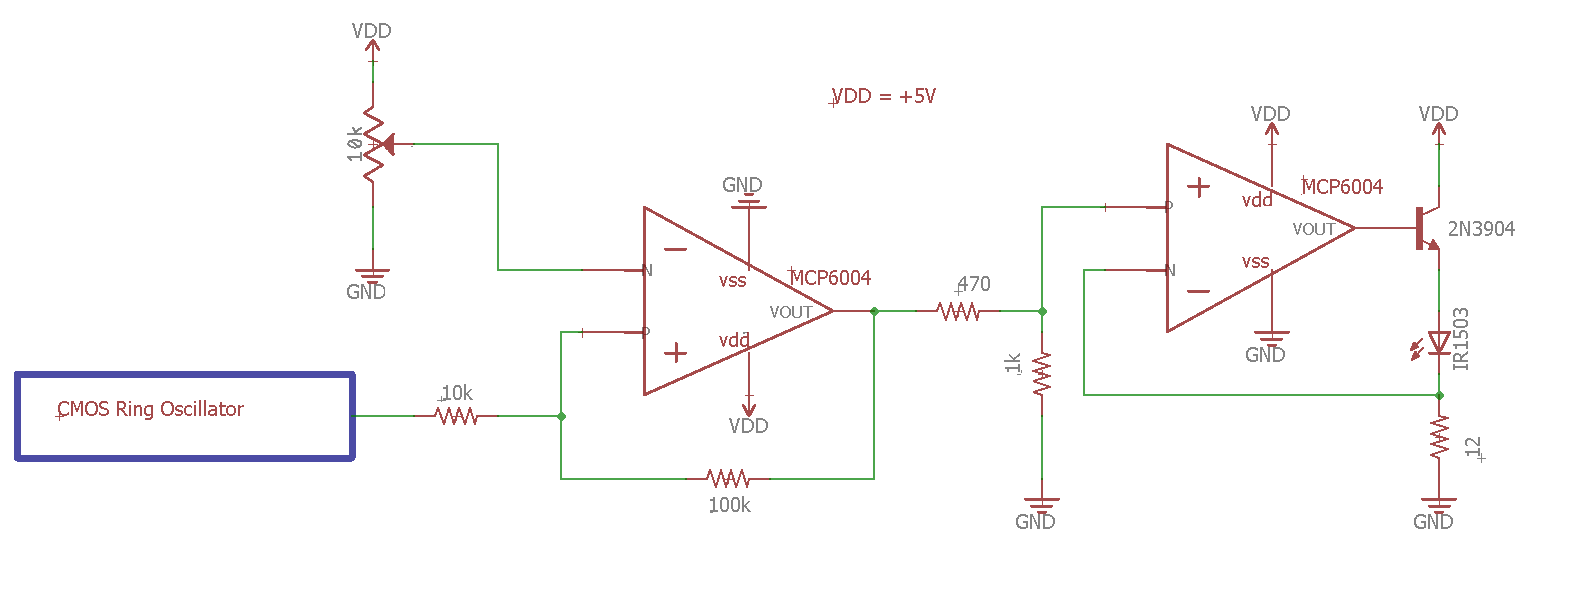
\includegraphics[width=0.7\linewidth]{Preliminary_results/FINAlexperimentalSchem}
	\caption{Circuit schematic of transmitter}
	\label{fig:finalexperimentalschem}
\end{figure}

The astable multivibrator is constructed on a signal CD4007 MOS DIP, which consists of three CMOS circuits. The waveform is then conditioned with a Schmitt trigger and then passed through a amplifier, both constructed on an MCP6004 quad-op-amp. This, in turn, drives an 2N3904 BJT, which controls the current through the IR1503 LED. The resulting current is seen in Figure \ref{fig:expcurrentlab4}.

\begin{figure}[H]
	\centering
	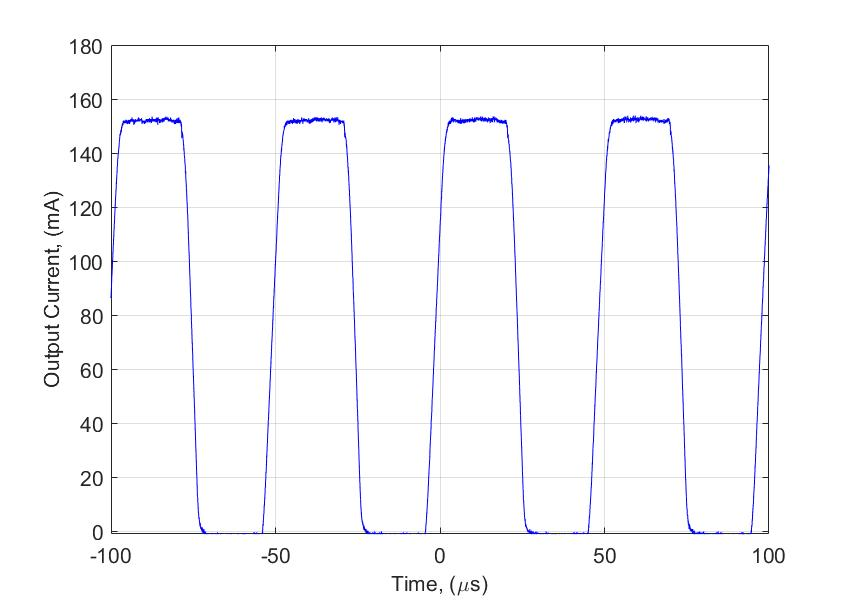
\includegraphics[width=0.7\linewidth]{Preliminary_results/expcurrentlab4}
	\caption{Current through LED}
	\label{fig:expcurrentlab4}
\end{figure}

The maximum current was found to be 150mA, with a duty-cycle of 50\%. This current for the LED is important for energy conservation regions and to not overheat the IR LED. The LED will not overheat in this manner, which will also prevent parasitic effects of temperature change from affecting it. This results in steady operation of the system as a whole, which will in turn provide accurate results of foot traffic in stores. 


	
\end{document}